\section{Ejercicio 4 - Usar el cálculo con nombre para los nombres de miembro}  

1. Haga doble clic en la dimensión DimDate en el nodo Dimensiones del Explorador de soluciones.

2. En el panel Atributos de la pestaña Estructura de dimensión, haga clic en el atributo Date Key

	\begin{center}
	
\includegraphics[width=\columnwidth]{images/task4/img1}
	\end{center}	

3.Haga clic en el campo de la propiedad NameColumn y, a continuación, haga clic en el botón de puntos suspensivos
(…) para abrir el cuadro de diálogo Columna de nombre.
	\begin{center}
	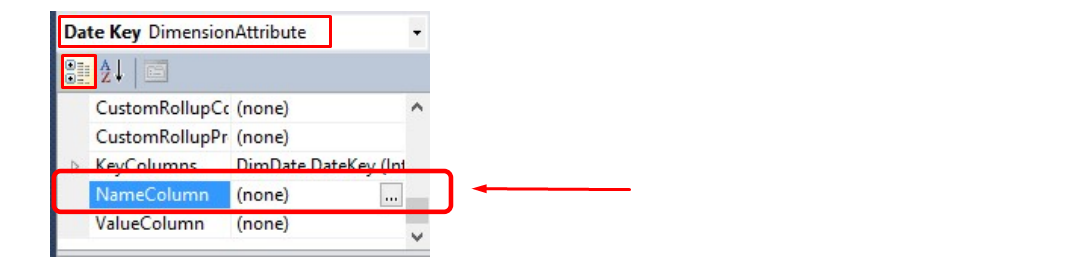
\includegraphics[width=\columnwidth]{images/task4/img2}
	\end{center}	

4. Seleccione SimpleDate en la lista Columna de origen y, a continuación, haga clic en Aceptar.

	\begin{center}
	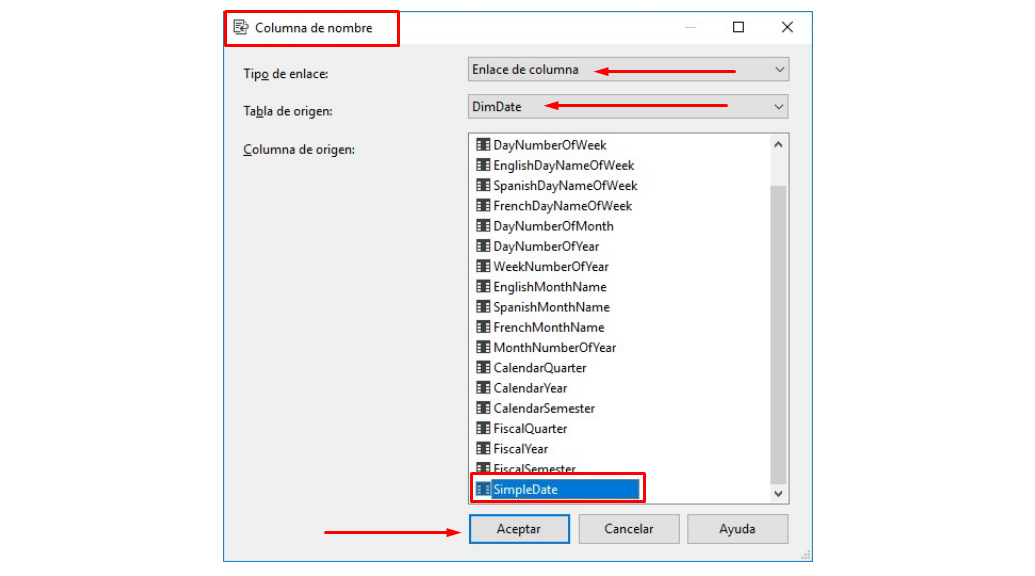
\includegraphics[width=\columnwidth]{images/task4/img3}
	\end{center}	

5. En el menú Archivo del proyecto, haga clic en Guardar todo

    